18. \begin{figure}[ht!]
\center{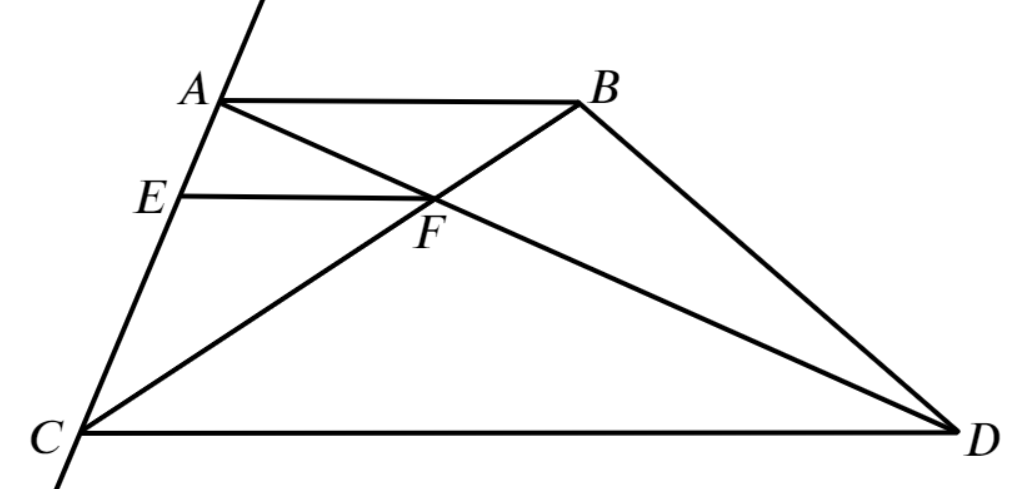
\includegraphics[scale=0.35]{g9-18.png}}
\end{figure}\\
Треугольники $ABF$ и $DCF$ подобны по двум углам ($\angle FAB=\angle FDC$ и $\angle FBA=\angle FCD$ как накрест лежащие), значит $\cfrac{BF}{CF}=\cfrac{AB}{CD}.$ Треугольники $CEF$ и $CAB$ также подобны по двум углам ($\angle CEF=\angle CAB$ и $\angle CFE=\angle CBA$ как соответственные), значит $\cfrac{CB}{CF}=\cfrac{AB}{EF}\Rightarrow \cfrac{CF+BF}{CF}=\cfrac{AB}{EF}\Rightarrow 1+\cfrac{AB}{CD}=\cfrac{AB}{EF}
\Rightarrow \cfrac{1}{AB}+\cfrac{1}{CD}=\cfrac{1}{EF},$ ч.т.д.\\
